\chapter{Preliminaries}

In this chapter a simple model will capture the relation between power harvested and distance covered by the robot.
The design considerations for the robot will be explained based on minimal required capabilities. 
Followed by an evaluation of stepper motor based locomotion for a transiently powered robot.

% RF harvesting seems prommesing
% Wispcam requires approx 4 seconds to harvest 20mJ at a distance of 20cm from the reader \cite{naderiparizi_rfid_2015}
% better to only use RF for communication and harvest energy from another source \cite{konstantioulos}

% Energy can be harvested from different sources

\section{Energy Source Selection}

\subsection{Energy Harvesting from RF}

% Remove robot part from this ??
% Do same process with bq25570 evaluation board from ti

%TODO explain that the it's more efficient to remove the wisp energy harvester and only use the one on the robot
\subsubsection{Experimental Setup}

Small modifications have been made to the WISP to allow the energy harvester on the robot to harvest energy from RF.
The energy harvester, the storage capacitor and the diode to bypass the harvester, were removed from a WISP.
A wire was soldered to the input pin pad of the now removed harvester on the WISP PCB.
This wire was connected directly to the input of the harvester on the robot.

To evaluate the time required for the robot to harvest enough energy the following experiment was done.
Energy was provided to the WISP on the robot trough an Impinj Speedway R1000 RFID reader, which was connected to a Laird S90028PCR antenna.

\subsubsection{Results}
The robot was placed 20 cm away from the antenna, typically the distance where the most energy is harvested.
On average the robot required 48 seconds fully charge and move away from the reader.

\subsubsection{Energy Harvesting from Light}
% Casestudy of conditions robot 
% outdoors/indoors/varying light sources/varying solar panels
% Do experiment in sunlight for nuna panel

%The amount of energy that can be harvested from normal office lighting is limited.
In this section the charge time of the supercapacitor is evaluated, while it's charged from different solar panels and different light sources.
Currently the robot harvests energy form light using a small solar panel.
However, there is not always enough sunlight available to charge the robots in a acceptable time.
To allow the robots to have sub ten seconds charge times, a lighting setup needs to be created that provides a reasonable amount of uniform light to the area where the robots move around.


\subsubsection{Experimental setup}
% Temperature and Light intensity?
To accurately measure the power that is harvested from each solar panel all the experiments were preformed in a darkroom at TU Delft Embedded Software Lab.
The setup consists of a light source that can be positioned at multiple distances from a solar panel.
The solar panel is connected to input of the harvester on the PCB of the robot and when the voltage in the supercapacitor reaches the threshold the buck converter of the energy harvester is enabled.
Voltage is supplied to the WISP which is programed to only enable a GPIO port and enable a LED.
A Saleae Logic, logic analyzer is connected to the port and used to record the time required to charge the capacitor from the minimum to the maximum value.
The port is enabled the light source is disabled and the LED is used to drain the energy from the capacitor.
When the led turns off, indicating that a new charge period begins, the light source is enabled again.
A more detailed description will be given of the different components that were tested.

\textit{Solar panels}
Three different solar panels were tested in this experiment, each different in composition, efficiency and panel size, as can be seen from Table \ref{tab:solar_panels}.

%TODO Why these lamps?
\textit{Lamps}
Low cost solar simulators can consist of a combination of LED and halogen light bulbs to simulate sunlight and are used to test the performance of solar panels~\cite{grandi_tia_2014}.
However, in this case the goal is to have a controlled uniform lighting environment where the robots have roughly constant charge times.
Solar panels do not only harvest energy from the visual light spectrum but harvest almost at least as much from the infrared light spectrum, therefore not only light but also heat will shorten the charge time.
Halogen lamps have a lower color temperature than the sun but also emit waves far into the infrared spectrum.
The light sources used in this experiment are a 60 W halogen bulb, a 120 W halogen halogen bulb and two 150 W IR heat lamps where one is colored red.

\textit{Measurements}
Three charge time measurements were preformed, each lamp was positioned 10 cm, 30 cm and 50 cm from the solar panels.
Additionally, for these three distance the temperature was measured at the solar panel using a K-type thermocouple supplied with an Extech EX330 multimeter and the light intensity using the luxmeter on a MASTECH MS8229 multimeter.

\begin{table}[t]
	\centering
	\begin{threeparttable}
		\caption{Specification of the solar panels tested in the experiment.}
		\label{tab:solar_panels}
		\small
		\begin{tabular}{|l|l|l|l|}
			\hline
			& Material & Efficiency (\%) & Dimensions (mm) \\
			\hline \hline
			Banggood \cite{bangood_solar_2017}& Poly-Si & 17 & 40x30 \\
			INYS SLMD121H04L-ND\textsuperscript{1}& Mono-Si & 22 & 43x34 \\
			Azurspace 3G28C & Triple Junction GaAs& 28 & 80x40 \\
			\hline
		\end{tabular}
		\begin{tablenotes}
			\small
			\item [1] Two panels in parallel
		\end{tablenotes}
	\end{threeparttable}
\end{table}

\subsubsection{Results}
% No difference between the heatlamps in power consumed
% Halogen distributes the light more even
% Panel from nuna
% Refer to appendix for temperature and light data?

Both the temperature and illumination increase by decreasing the distance between the light source and the solar panel. 
Secondly, increasing the output power of the lamp increases temperature and illumination as well. 
However the charge times 
A thing to note is that the both the 60 W and 150 W IR lamps have a spherical design. This creates a uneven circular shadowing pattern on the surface the lamps are shining on, which becomes more significant on the bigger distances in this experiment.
The 120 W halogen lamp has a tubular design and in combination with the light fixture most of the light is reflected down with minimal shadowing of the lamp resulting in a more even light distribution.

\begin{figure}
	\centering
	\begin{subfigure}[b]{0.62\textwidth}
		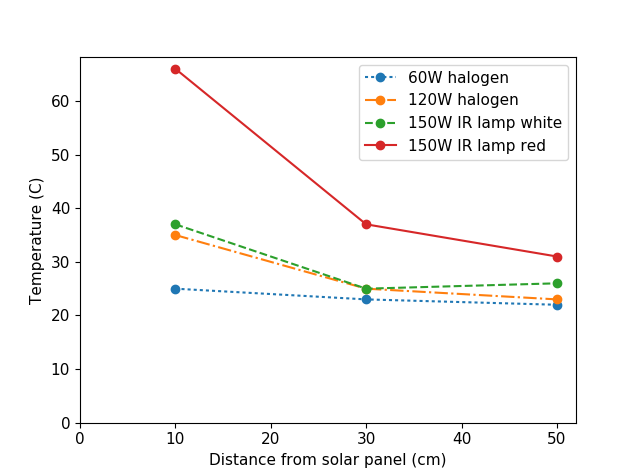
\includegraphics[width=\textwidth]{pics/light_experiment_temp.png}
		\caption{Temperature at different distances}
		\label{fig:light_temp}
	\end{subfigure}
	\begin{subfigure}[b]{0.62\textwidth}
		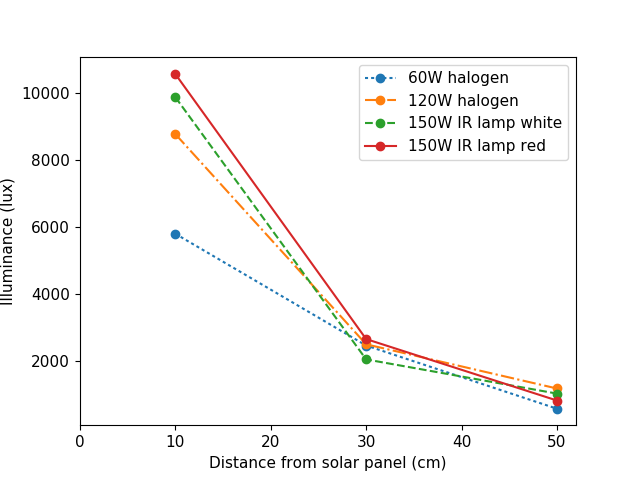
\includegraphics[width=\textwidth]{pics/light_experiment_lux.png}
		\caption{Light intensity at different distances}
		\label{fig:light_lux}
	\end{subfigure}
	\caption{}
\end{figure}


\begin{figure}
	\centering
	\begin{subfigure}[b]{0.62\textwidth}
		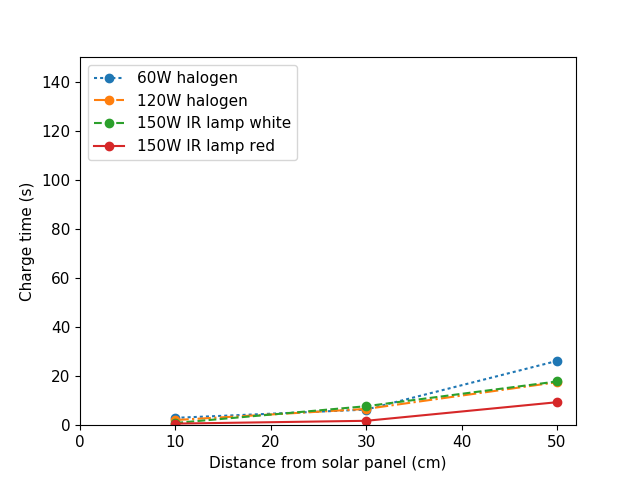
\includegraphics[width=\textwidth]{pics/light_experiment_figure1.png}
		\caption{Ebay panel}
		\label{fig:light_exp1}
	\end{subfigure}
	\begin{subfigure}[b]{0.62\textwidth}
		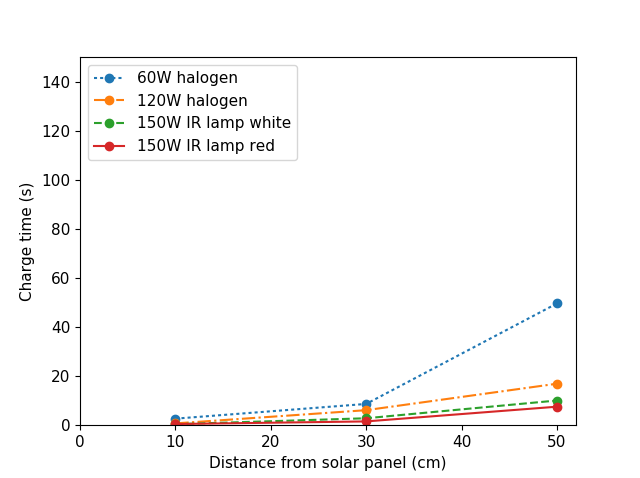
\includegraphics[width=\textwidth]{pics/light_experiment_figure2.png}
		\caption{IXYS SLMD121H04L-ND}
		\label{fig:light_exp2}
	\end{subfigure}
	\begin{subfigure}[b]{0.62\textwidth}
		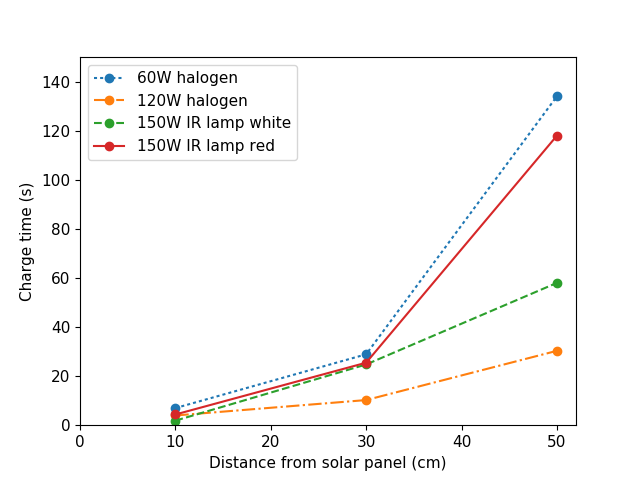
\includegraphics[width=\textwidth]{pics/light_experiment_figure3.png}
		\caption{Azurspace 3G28C}
		\label{fig:light_exp3}
	\end{subfigure}
	\caption{The performance of three different solar panels for different distances from different light sources. The data charge times for the last two are normalized with respect to the surface covered by the first panel.}
\end{figure}

\section{Locomotion Selection}

\subsection{Stepper motor-based Locomotion}

In order for a robot to move between locations without external feedback, accurate locomotion and basic odometry are required.
%TODO DEFINE AND REFERENCE
Wheel encoders are often used to determine the angular speed of each wheel, which can be used to correct speed differences between the motors and can be integrated over time to acquire distance.
Miniaturizing encoders significantly reduces their resolution, and can be classified as power hungry when considering a small energy budget and active light source is used.
%TODO NEED REFERENCE FOR THIS CLAIM
The GRITSBot~\cite{pickem_icra_2015} uses stepper motors to achieve accurate locomotion and basic odometry, as described in Section \ref{sec:locomotion}.
This section will further investigate the use of stepper motor based locomotion in combination with a transiently-powered robot.

\subsubsection{Operation of a Stepper Motor}
Stepper motors are permanent magnet dc motors that start to rotate by supplying current to the motor coils in a specific direction.
The bipolar stepper motor used, requires current to be pulsed trough each of the four connections, in a fixed pattern, in order to rotate it forward or backward.
A Microcontroller (MCU) is used to keep track and instruct the next stepper motor position from a sequence of four.
The outputs of the MCU cannot supply enough current to drive a bipolar stepper motor, therefore a dual H-bridge is required to control the current trough each coil.

%TODO make new schematic stepper figure!
%http://homemaderobo.blogspot.nl/2012/03/stepper-motor.htm
\begin{figure}
	\centering
	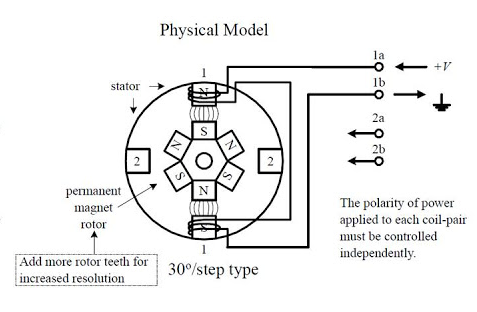
\includegraphics[width=\textwidth]{pics/bipolar_stepper.png}
	\caption{Need better / simpler figure here!}
	\label{fig:bipolarstepper}
\end{figure}

\subsubsection{Power Consumption}
%TODO values that calculate the current per motor?
%TODO ADD CURRENT MEASUREMENTS @ 2.2 v
The current consumed by a stepper motor is constant and independent of the angular velocity of the motor.
The average current consumed is equal to: $\textrm{I} = V_{\text{supply}}/R_{\text{coil}}$.
Therefore running the motor at maximum speed, translates the most electrical energy into kinetic energy.
However, the motor speed is inversely proportional to the motor's output torque and therefore the maximum speed is limited by the minimal required output torque.
%The current trough the coils is constant, so the faster the stepper motor changes step the more energy can be transformed into movement.
%Increasing the rotational speed of the stepper motor decreases the torque output of the motor.
%Therefore the speed is limited by the amount of torque required to preform the movement.

\subsubsection{Control and Rotor Synchronization}

The only way to grantee that the teeth on the rotor will stay aligned with the coil, is to keep the coil energized until the next position is instructed and succeeding coil is energized. 
On the first startup the rotor may not be aligned with the last position in the sequence of four.
As a result an error between one and three steps can occur before the energized coil and rotor are synchronized.

In case the stepper motor is rotating and the power is removed, misalignment between the rotor and the last energized coil can occur.
While the rotor could be moving from one position to the next, it has not moved at all (undershoot) or can continue to move to the next position due to inertia of the rotating mass (overshoot). 
To determine what would be more likely, undershooting or overshooting, the following experiment has been preformed to determine the error in the number of steps.

\subsubsection{Experimental setup}

Tiny permanent magnet bipolar stepper motors can be sourced from Ebay.com, while they are frequently used in digital camera's~\cite{nidec_stepper_2017}.
A stepper motor is suspended and a needle glued to the motor shaft.
The needle rotates over a round piece of paper which is divided by markings in 20 steps, as seen from Figure \ref{fig:step_counting}.
First the rotor and coil are synchronized by moving four steps, and the position of the needle is visually recorded and written down.  
Then the stepper motor is commanded to make one rotation equal to 20 steps.
After rotating 20 steps the power is removed from the coils and the needle position recorded when the needle is not rotating anymore.

\begin{figure}
	\centering
	\begin{subfigure}[b]{0.38\textwidth}
		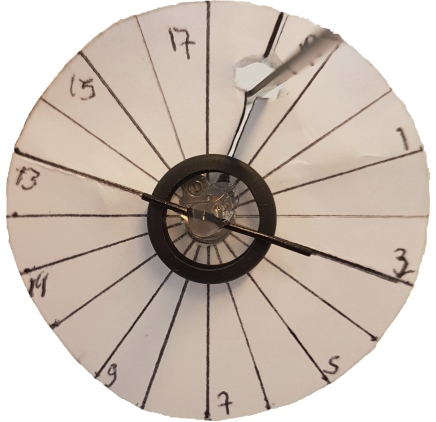
\includegraphics[width=\textwidth]{pics/step_counting.jpg}
		\caption{Experimental setup for determining error in the number of counted steps}
		\label{fig:step_counting}
	\end{subfigure}	
	\quad
	\begin{subfigure}[b]{0.55\textwidth}
		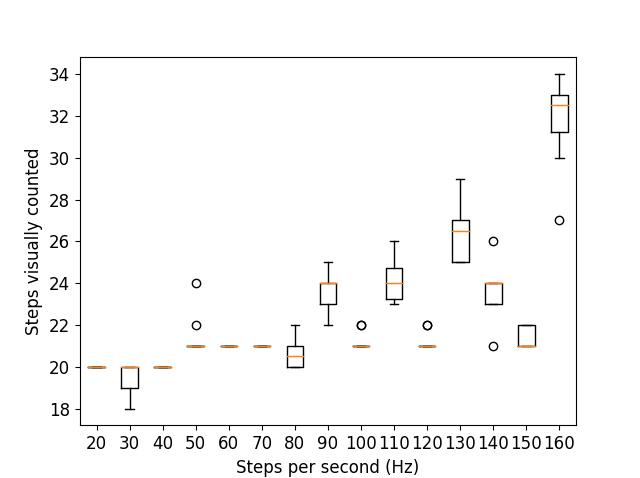
\includegraphics[width=\textwidth]{pics/figure_intertia.png}
		\caption{}
		\label{fig:step_results}
	\end{subfigure}
	\caption{}
\end{figure}

\subsubsection{Stepper Motor Inertia Result}

Figure \ref{fig:step_results} shows the result of the experiment.
The stepper motor on average will overshoot, i.e. will do more steps than commanded when the power is removed.
This effect is becomes more significant with increasing step frequency or speed of rotation.
However, while this experiment only shows the effect for an unloaded motor, it is likely that a synchronization error will occur when a transiently-powered robot would be powered using two stepper motors in differential drive.
After every power interrupt each motor first needs to be synchronized, which will result in the robot making a turn if the error between the motors is not equal.

%TODO Write conclusion here! + link to rest of thesis

\subsection{DC Motor locomotion}

%TODO expain the general operation of a dc motor!
%TODO tell something about the motors considered
%TODO Show measurement / current profile of a dc motor


%TODO tell something about the maximum speed that can be achieved

On average the each motor consumes 38 mA while running on a flat surface, which is well within the current limit that the buck converter can supply.
However when the motors are in not moving yet the start current is approximately equal to the stall current, which is equal to 240 mA.
This amount of current can not be supplied by a most regulators, PWM can be used to reduce the average current allowing a bulk capacitor to supply the voltage.


\section{Transiently-powered Robot Model}
\label{sec:transient_model}

In this section a simple model will be derived showing the relation between size and weight of the robot, the amount of power that is harvested and stored and how much of this can be translated into linear movement.

\subsection{Modeling Assumptions}

Energy is harvested from an ambient source and stored in a supercapacitor.
To make efficient use of the energy stored in a supercapacitor a regular is required to supply a stable voltage to the connected loads.
In this case the loads are two identical dc motors which each drive wheel. \\
\\ \noindent
The following assumptions will be used to model the transiently powered robot:
\begin{itemize}
	\item The required power by the loads is greater than the incoming power, resulting in repeated power cycling of the robot.
	\item The amount of input power after conversion is constant due to the use of a controlled environment
	\item Since a regulator is used, the voltage in the capacitor will never fall below the operating voltage.
\end{itemize}

%The input power Pin, will be stored in a supercapacitor with capacitance C.


%The regulated output voltage is a lower threshold for the energy that can be used from the capacitor.
%The upper threshold is determined by the maximum voltage rating of the supercapacitor.
%Lowering the output voltage allows for more energy to be used from the supercapacitor, and also lowers the overall power consumption of individual components.
%The energy stored in supercapacitor is a function of the capacitance and the threshold voltage difference, being equal to:

\begin{equation}
\label{eq:cap2}
E = \frac{1}{2}C(V_{\max} - V_{\min})^{2}
\end{equation}






% 1 Incomming power V * I which scales with solar panel size

% 2 Maximum power point tracking (switchmode boost converter)

% 3 Stored in non-ideal supercapacitor with capcitiy C and a parrallel resistance Rleak and series resistance (ESR, typically small but not neglectable?)

% 123 determine chargetime

% Buck converter losses 

% Power consumed from source = Pcons = Ploss + Pweels

% Power P(t)  = F * v = T x omega

\subsection{Motor Dynamics}

\begin{circuitikz}
	%	\draw [help lines] (-1,-2) grid (12,5);
	
	% electrical equivalent circuit
	\draw (0,0) to[V, v_=$v$] (0,3);
	\draw (0,3) to[R, i>^=$i$, l=$R$] (3,3);
	\draw (3,3) to[L, l=$L$] (4,3);
	
	\draw (4,3) -- (5,3);
	\draw (5,0) to[V, v_=$U_i$] (5,3);
	\draw (0,0) -- (5,0);
	
	% drive
	\draw[fill=white] (4.85,0.85) rectangle (5.15,2.15);
	\draw[fill=white] (5,1.5) ellipse (.45 and .45);
	
	% shaft drive -> transmission
	\draw[fill=black] (5.45,1.45) rectangle (6.5,1.55);
	
	% momentum arrow of drive -> transmission
	\draw[line width=0.7pt,<-] (5.8,1) arc (-30:30:1);
	
	% moment of inertia
	\draw[fill=white] (7.5,1.59)
	ellipse (.15 and 0.4);
	\draw[fill=white, color=white] (6.9, 1.99)
	rectangle (8.49, 1.19);
	\draw (6.8,1.59) ellipse (.15 and 0.4);
	\draw (6.8,1.99) -- (7.5,1.99);
	\draw (6.8,1.19) -- (7.5,1.19);
	
	% shaft right from moment of inertia
	\draw[fill=black] (8.65,1.55) rectangle (8.9,1.65);
	
	% momentum arrow (left hand side of brake shoe)
	\draw[line width=0.7pt,->] (8.05,1.1) arc (-30:30:1);
	
	% descriptions inside graphic
	\draw (5.85,2.2) node {$\omega_A, M_A$};
	\draw (7.25,1.61) node {$J$};
	\draw (8.05,2.32) node {$M_R$};
	
\end{circuitikz}
\\
\noindent
The electrical dynamics of a dc motor can be described as:
\begin{equation}
v = Ri + L \dot{i} + e
\end{equation}

\noindent
The mechanical dynamics of a motor can be described as:
\begin{equation}
\tau = J\dot{\omega} + B\omega + m
\end{equation}

\noindent
The electromechanical equations state that the back emf voltage is proportional to the angular velocity and the motor torque is proportional to the armature current:

\begin{equation}
\begin{gathered}
e = k_{e} \omega \\
\tau = k_{t} i
\end{gathered}
\end{equation}

\noindent
The electrical power consumed and mechanical power consumed will be equal to:

\begin{equation}
\begin{gathered}
p_{\text{e}} = vi \\
p_{\text{m}} = \tau\omega
\end{gathered}
\end{equation}


\subsection{Robot Dynamics}
The robot is modeled as a mass $m$, that is moved by two wheels with radius $r$, each connected directly to a motor.


The rolling friction between the wheels and the surface is equal to:
\begin{equation}
F_{\text{k}} = \mu_{\text{k}}mg
\end{equation}

Therefore the torque applied to the motor due to rolling friction, as it is only present while the robot is moving relative to the surface and the equation becomes:

\begin{equation}
T_{\text{ext}} = rF_{\text{k}} sgn(\omega)
\end{equation}

\noindent
The total mass is equal to the 



\section{Design Considerations}
\label{sec:design_considerations}

This section will shortly explain the main areas considered while designing the battery-less transiently-powered robot

% - Optimize or low power consumption (disable or standby sensors and motor ctrl when not used)
% - Minimal basic functionality (for simple swarm algorithms?) (but no power hungry components ie optical encoders or mouse sensors)
% - Low power communication
% - Navigation

% Extra extra:
% - Tradeoff chargetime and operation time

\begin{enumerate}
	\item \textbf{Power}. 
	The robot should not rely on batteries, alternatively energy can be harvested from ambient sources and stored in a supercapacitor. 
	Energy harvested in a controlled environment should charge the capacitor in under 10 seconds and stored energy should provide at least an operation time of 1 second, allowing the robot to make short controlled movements.
	
	\item \textbf{Small form factor}. 
	By making the robot as small as possible, weight is kept to a minimum reducing the energy required for movement.
	Secondly, by design the robot using low cost off-the-shelf parts, should make it convenient to build collectives of transiently-powered robots.
	
	\item \textbf{Locomotion}.
	Movement will consume the largest amount of energy from the total available energy budget.
	To optimize the distance that can be covered with a single capacitor charge, an efficient locomotion type should be chosen for the movement on flat surfaces.
	
	\item \textbf{Autonomous navigation}.
	During operation the robot will experience a very frequent loss of power. 
	Despite regular power interruption the transiently-powered robot should be able to complete a movement with an acceptable error compared to the same robot being battery powered.
	
	%TODO write about ability to expand to swarming
\end{enumerate}
